% Options for packages loaded elsewhere
\PassOptionsToPackage{unicode}{hyperref}
\PassOptionsToPackage{hyphens}{url}
%
\documentclass[
  ignorenonframetext,
]{beamer}
\usepackage{pgfpages}
\setbeamertemplate{caption}[numbered]
\setbeamertemplate{caption label separator}{: }
\setbeamercolor{caption name}{fg=normal text.fg}
\beamertemplatenavigationsymbolsempty
% Prevent slide breaks in the middle of a paragraph
\widowpenalties 1 10000
\raggedbottom
\setbeamertemplate{part page}{
  \centering
  \begin{beamercolorbox}[sep=16pt,center]{part title}
    \usebeamerfont{part title}\insertpart\par
  \end{beamercolorbox}
}
\setbeamertemplate{section page}{
  \centering
  \begin{beamercolorbox}[sep=12pt,center]{part title}
    \usebeamerfont{section title}\insertsection\par
  \end{beamercolorbox}
}
\setbeamertemplate{subsection page}{
  \centering
  \begin{beamercolorbox}[sep=8pt,center]{part title}
    \usebeamerfont{subsection title}\insertsubsection\par
  \end{beamercolorbox}
}
\AtBeginPart{
  \frame{\partpage}
}
\AtBeginSection{
  \ifbibliography
  \else
    \frame{\sectionpage}
  \fi
}
\AtBeginSubsection{
  \frame{\subsectionpage}
}

\usepackage{amsmath,amssymb}
\usepackage{lmodern}
\usepackage{iftex}
\ifPDFTeX
  \usepackage[T1]{fontenc}
  \usepackage[utf8]{inputenc}
  \usepackage{textcomp} % provide euro and other symbols
\else % if luatex or xetex
  \usepackage{unicode-math}
  \defaultfontfeatures{Scale=MatchLowercase}
  \defaultfontfeatures[\rmfamily]{Ligatures=TeX,Scale=1}
\fi
% Use upquote if available, for straight quotes in verbatim environments
\IfFileExists{upquote.sty}{\usepackage{upquote}}{}
\IfFileExists{microtype.sty}{% use microtype if available
  \usepackage[]{microtype}
  \UseMicrotypeSet[protrusion]{basicmath} % disable protrusion for tt fonts
}{}
\makeatletter
\@ifundefined{KOMAClassName}{% if non-KOMA class
  \IfFileExists{parskip.sty}{%
    \usepackage{parskip}
  }{% else
    \setlength{\parindent}{0pt}
    \setlength{\parskip}{6pt plus 2pt minus 1pt}}
}{% if KOMA class
  \KOMAoptions{parskip=half}}
\makeatother
\usepackage{xcolor}
\newif\ifbibliography
\setlength{\emergencystretch}{3em} % prevent overfull lines
\setcounter{secnumdepth}{-\maxdimen} % remove section numbering


\providecommand{\tightlist}{%
  \setlength{\itemsep}{0pt}\setlength{\parskip}{0pt}}\usepackage{longtable,booktabs,array}
\usepackage{calc} % for calculating minipage widths
\usepackage{caption}
% Make caption package work with longtable
\makeatletter
\def\fnum@table{\tablename~\thetable}
\makeatother
\usepackage{graphicx}
\makeatletter
\def\maxwidth{\ifdim\Gin@nat@width>\linewidth\linewidth\else\Gin@nat@width\fi}
\def\maxheight{\ifdim\Gin@nat@height>\textheight\textheight\else\Gin@nat@height\fi}
\makeatother
% Scale images if necessary, so that they will not overflow the page
% margins by default, and it is still possible to overwrite the defaults
% using explicit options in \includegraphics[width, height, ...]{}
\setkeys{Gin}{width=\maxwidth,height=\maxheight,keepaspectratio}
% Set default figure placement to htbp
\makeatletter
\def\fps@figure{htbp}
\makeatother

\makeatletter
\makeatother
\makeatletter
\makeatother
\makeatletter
\@ifpackageloaded{caption}{}{\usepackage{caption}}
\AtBeginDocument{%
\ifdefined\contentsname
  \renewcommand*\contentsname{Table of contents}
\else
  \newcommand\contentsname{Table of contents}
\fi
\ifdefined\listfigurename
  \renewcommand*\listfigurename{List of Figures}
\else
  \newcommand\listfigurename{List of Figures}
\fi
\ifdefined\listtablename
  \renewcommand*\listtablename{List of Tables}
\else
  \newcommand\listtablename{List of Tables}
\fi
\ifdefined\figurename
  \renewcommand*\figurename{Figure}
\else
  \newcommand\figurename{Figure}
\fi
\ifdefined\tablename
  \renewcommand*\tablename{Table}
\else
  \newcommand\tablename{Table}
\fi
}
\@ifpackageloaded{float}{}{\usepackage{float}}
\floatstyle{ruled}
\@ifundefined{c@chapter}{\newfloat{codelisting}{h}{lop}}{\newfloat{codelisting}{h}{lop}[chapter]}
\floatname{codelisting}{Listing}
\newcommand*\listoflistings{\listof{codelisting}{List of Listings}}
\makeatother
\makeatletter
\@ifpackageloaded{caption}{}{\usepackage{caption}}
\@ifpackageloaded{subcaption}{}{\usepackage{subcaption}}
\makeatother
\makeatletter
\@ifpackageloaded{tcolorbox}{}{\usepackage[many]{tcolorbox}}
\makeatother
\makeatletter
\@ifundefined{shadecolor}{\definecolor{shadecolor}{rgb}{.97, .97, .97}}
\makeatother
\makeatletter
\makeatother
\ifLuaTeX
  \usepackage{selnolig}  % disable illegal ligatures
\fi
\IfFileExists{bookmark.sty}{\usepackage{bookmark}}{\usepackage{hyperref}}
\IfFileExists{xurl.sty}{\usepackage{xurl}}{} % add URL line breaks if available
\urlstyle{same} % disable monospaced font for URLs
\hypersetup{
  hidelinks,
  pdfcreator={LaTeX via pandoc}}

\author{}
\date{}

\begin{document}
\ifdefined\Shaded\renewenvironment{Shaded}{\begin{tcolorbox}[borderline west={3pt}{0pt}{shadecolor}, sharp corners, enhanced, breakable, interior hidden, frame hidden, boxrule=0pt]}{\end{tcolorbox}}\fi

\begin{frame}
https://arxiv.org/abs/2204.00227
\end{frame}

\begin{frame}[fragile]{Background}
\protect\hypertarget{background}{}
First, a bit of review. Each \(x_t\) is dependent on some \(x_{t-1}\) in
a Markov chain defined below. This we can also define in terms of
\(a_t\) and \(x_0\), so that we can calculate the amount of noise at
each step without the calculation being Markovian(or dependent on the
previous step). This essentially gives us a formula that is the original
image \(x_0\) plus some noise \(\epsilon\)

\(q(x_t|x_{t-1}) = \mathcal{N}(x_t;\sqrt{1-\beta_t}x_{t-1},\beta_t\textbf{I})\\ \epsilon\sim\mathcal{N}(0,\textbf{I})\\ a_t := \prod_{s=1}^t{1-\beta_s}\\ x_t = \sqrt{\alpha_t}x_0+\sqrt{1-\alpha_t}\epsilon\)

Both \(\alpha_t\) and \(\beta_t\) are of interest to us, so we define
the code here. We have 1000 values, one value for each time step \(t\).

\begin{verbatim}
torch.Size([1000])
\end{verbatim}

Signal-to-noise ratio is very important for this paper. We if we put the
below two formulas close together the relationship should be clear,
remembers that \(x_0\) is the original image, and \(\epsilon\) is our
noise.

\(x_t = \sqrt{\alpha_t}x_0+\sqrt{1-\alpha_t}\epsilon\\ SNR(t) = \frac{\alpha_t}{1-\alpha_t}\)

Another noise schedule that is investigated is the cosine noise
schedule, we define the code for it below.

We can now take a look at the noise schedule per diffusion step \(t\).
Remeber low \(\alpha_t\) means more noise \(\epsilon\).

\begin{verbatim}
<matplotlib.legend.Legend at 0x7fd7e2d69870>
\end{verbatim}

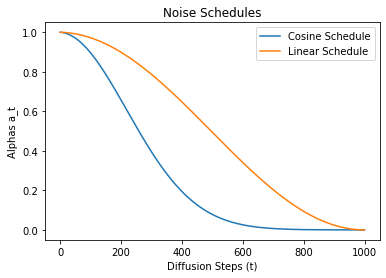
\includegraphics{Perception Prioritized Training of Diffusion Models_files/figure-beamer/cell-7-output-2.png}

Now we can graph the signal to noise ratio for both the cosine and
linear schedules.

\begin{verbatim}
<matplotlib.legend.Legend at 0x7fd8e86670a0>
\end{verbatim}

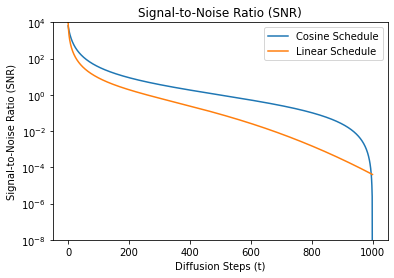
\includegraphics{Perception Prioritized Training of Diffusion Models_files/figure-beamer/cell-8-output-2.png}

Notice that we get very similar results to the paper as seen below.

\begin{figure}

{\centering 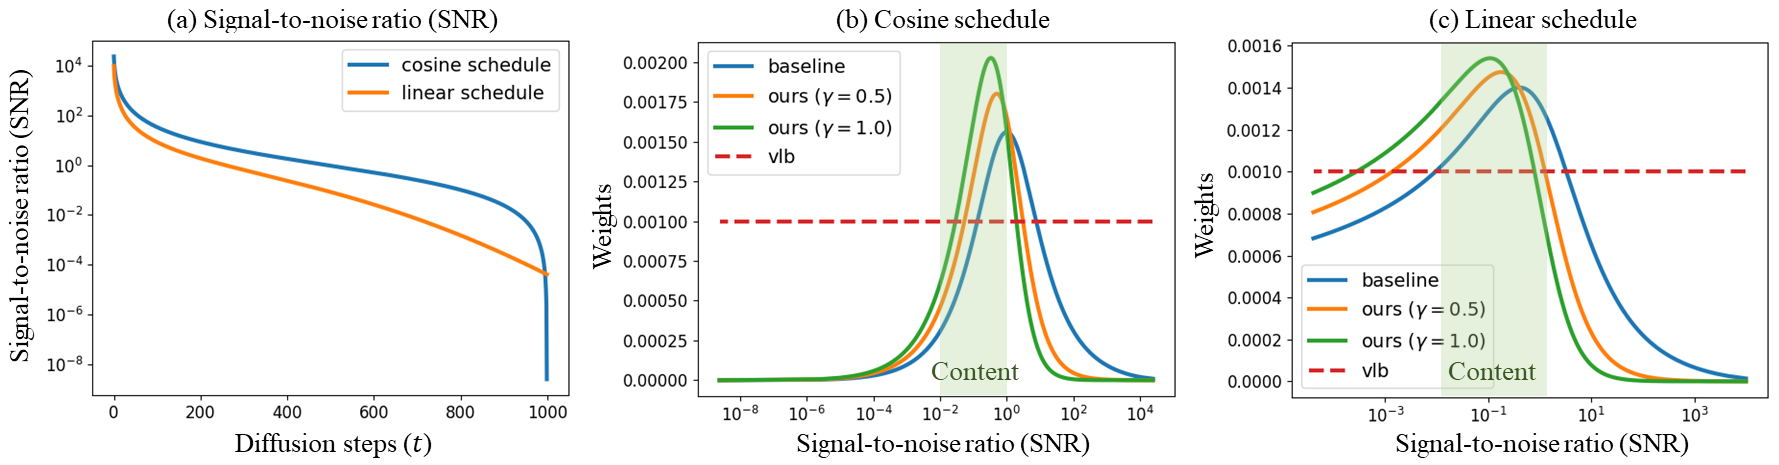
\includegraphics{Perception Prioritized Training of Diffusion Models_files/figure-beamer/161203299-8b02d76b-9c51-4529-8329-3ac08e9f3bc8.png}

}

\caption{161203299-8b02d76b-9c51-4529-8329-3ac08e9f3bc8.png}

\end{figure}

Okay, now we need to determine the weights above. This is the goal of
the paper. First we look at the first contribution, a way to calculate
the weights in terms of the signal-to-weight ratio, which is a
continuous version of the weighting scheme introduced in the DDPM paper.
The derivation of this is in the paper's appendix.

We can now compare the unnormalized weights of the continuous weight
schedule and the one in the DDPM paper. They are fairly close.

\begin{verbatim}
<matplotlib.legend.Legend at 0x7fd7e2e0eb60>
\end{verbatim}

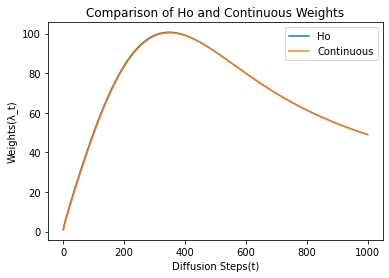
\includegraphics{Perception Prioritized Training of Diffusion Models_files/figure-beamer/cell-10-output-2.png}

Next we can look at the prioritized weight schedule. The main
contribution of the paper. \(\lambda_t\) is our continuous weights from
above, k is a constant set to \(1\). \(\gamma\) is a hyperparameter that
we can control, but it doesn't work so well at over 2, because ``We
empirically observed that γ over 2 suffers noise artifacts in the sample
because it assigns almost zero weight to the clean-up stage'' (quoting
paper).

\(\lambda_t^\prime = \frac{\lambda_t}{(k+SNR(t))^\gamma}\)

And, here is it in code. \(\gamma=0\) essentially turns the prioritized
weighting mechanism off, and gives us the same result as the weighting
mechanism in the DDPM paper.

Here we go ahead and generate weights based on a \textbf{linear} noise
schedule for different values of \(\gamma\). Notice how it is similar to
the results from the paper.

\begin{verbatim}
<matplotlib.legend.Legend at 0x7fd7e2a625c0>
\end{verbatim}

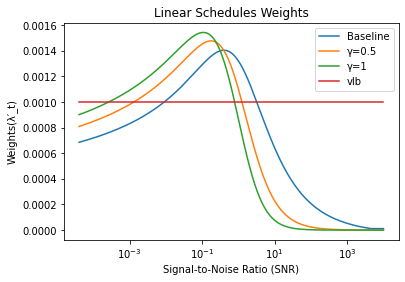
\includegraphics{Perception Prioritized Training of Diffusion Models_files/figure-beamer/cell-12-output-2.png}

Here we go ahead and generate weights based on a \textbf{cosine} noise
schedule for different values of \(\gamma\). Notice how it is similar to
the results from the paper.

\begin{verbatim}
<matplotlib.legend.Legend at 0x7fd7e2904d00>
\end{verbatim}

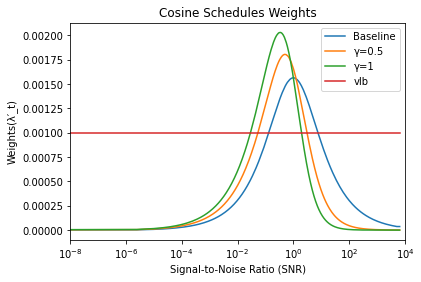
\includegraphics{Perception Prioritized Training of Diffusion Models_files/figure-beamer/cell-13-output-2.png}

Below you can see various results where the models performed better.
Note, on the right, the this paper's model is named P2. For the middle
table the schedule makes the most difference when a model is missing
attention, suggesting the weighting introduced helps with global
features. For the images, notice that the samples generated have better
clobal features, though both are going well at smaller details. The
authors believe this is because the weights help the model focus more on
global features.

\begin{figure}

{\centering 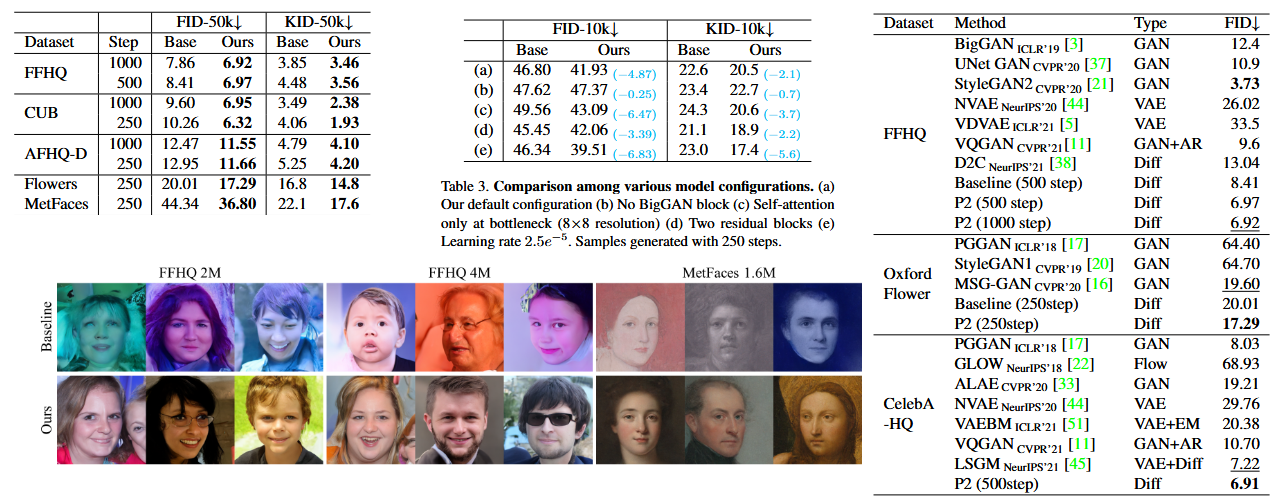
\includegraphics{Perception Prioritized Training of Diffusion Models_files/figure-beamer/paper_results.png}

}

\caption{paper\_results.png}

\end{figure}
\end{frame}



\end{document}
